\chapter{Causality Tracking}
\label{cha:causality-tracking}
This chapter, addresses the use of Bluetooth sightings as a way to
acquire knowledge about the movement patterns of people. To do so, we
propose a new technique with adjustable accuracy capable of
representing the causality relation between visited places. 

\section{Motivation and System Model}
\label{sec:ct-motivation}

The use of hash functions is often suggested as a data sanitation
technique in which the Bluetooth address is replaced by a digest from
which it is not be possible to recreate the original address. However,
this is also not suitable for large scale BT sensing, as it would be
possible, even with minimal information about someone, to identify the
respective digest, and from that point onward, the digest would again
function as a unique identifier (pseudonym).

There are examples, such as the Netflix
case~\cite{DBLP:journals/corr/abs-cs-0610105} that show how
surprisingly easy it can be to personalize information that was being
proposed as anonymous (\emph{quasi-identifier}
~\cite{bettini2005protecting}) simply by adding some basic additional
knowledge to the system. This is also visible in other
domains~\cite{Ohm:2010tc}. Therefore, the systematic registration of
Bluetooth sightings done at multiple locations constitutes a privacy
threat in that it allows the creation of a surveillance system for
people.

The use of Bluetooth as an enabling technology to establish the flows
of people is not a new concept. There are several examples, be it
within a city~\cite{Oneill:2006vq}, outdoor
festival~\cite{versichele2012use} or shopping mall
~\cite{millonig2008shadowing}.

The model in which we base our work assumes the existence of a network
of heterogeneous and autonomous nodes that collaborate in the
tracking process of Bluetooth devices. These nodes may have access to
various types of information about the devices: their MAC address, the
timestamp of the sighting, the type of Bluetooth protocols supported
by the devices, among others. 

Similarly to Gate Counting scenario in Chapter
\ref{cha:gate-counting}, there is the possibility of using preexisting
resources (nodes). As a consequence, our model does not impose
restrictions on the type of information registered by the
scanners. The nodes will continue to perform the same functions they
did before as a part system. Our concern is to the information that
might be exchanged by the nodes in the context of collective tracking
and to the privacy risks that might ensue such as the ability
to accurately follow the movement of a device and therefore of its
respective owner.

In their everyday life and depending on their specific needs, people
visit several different places. For instance, a person $P_1$ wants to
buy a new laptop. To do so, she visits store $S_1$ which does not have
the model she wants. She then visits store $S_2$ which is out of
stock and afterwards store $S_3$ where the price is a little
steep. She ends up buying the laptop in store $S_4$. To represent this
behavior we introduce the concept of \emph{mobility traces}. A
mobility trace is simply the representation of the places visited in the
order by which they were visited. In this specific case, the mobility
trace of $P_1$ is $MT_{P_1}=\{S_1,S_2,S_3,S_4\}$. Our mechanism
\emph{Precedence Filters}, allows the recording of information
relative to the individual traces of people, in a manner compatible
with plausible deniability. That information can later be
processed/mined to obtain more accurate data about the habits of the
aggregate of all individuals. For instance, in this example, the order
in which the stores where visited might be an indicator of their
reputation/popularity.

A common strategy that seeks to strengthen privacy is the restriction
of captured data to just the essential. In our specific case, the goal
is the detection of movement patterns between nodes. As such, the
ability to detect the same device on different nodes is paramount. To
minimize the amount of information collected, we can ignore
information such as the duration of the sightings, the timestamp in which
they occurred, the device name, supported Bluetooth protocols,
among others. We just need the device's MAC address.

Whenever a device is sensed, the sighting node records that event
locally. This information is then used in the computation of device
transitions between the system's multiple nodes. The place where that
computation takes place depends on the system's architecture. In a
centralized system, the computation has to be done in the server since
only it has enough information to do so. Each node only shares its
local information with the server. On the other hand, with a
decentralized architecture, the processing can be done locally by the
nodes. The local information each node possesses is shared with the other
nodes, thus allowing all the nodes to have access to the same
data. Both models have advantages and disadvantages. For instance, the
centralized approach is not fault tolerant, if the server crashes the
tracking system stops working. This does not happen in the
decentralized approach given that the same information is stored in
multiple nodes (redundancy). The system can keep on working even if
some of the nodes fail. Compared to the centralized version, the
decentralized model also has greater availability, result of the
information redundancy. However, as a consequence of the exchange of
information between all the nodes, the decentralized scenario has
a bigger burden on the network when compared to the centralized one. 


In order to achieve the goal we set ourselves and taking into account
the constrains presented by our model, our solution is based upon the
following set of assumptions:
\begin{itemize}
\item Even though we cannot make assumptions about how each individual
  node will handle the observed Bluetooth addresses, our solution
  should never require the Bluetooth address or any other information
  that could uniquely identify individuals to ever leave the sensing
  node.
\item No system element should at any given time have all the
  information necessary to accurately determine the path of a single
  individual.
\item The aggregate result that a node can create about the set of all
  visiting devices should be accurate enough to be useful in human
  mobility observation scenarios, e.g. most common paths, similarity
  level between places.
\item There are no communication failures in the system and the
  exchange of information between any two nodes is faster than the
  time it takes for a person to move between them. This ensures that
  the order in which the sightings are recorded is correct, i.e, when
  a person goes from place $A$ to place $B$, node $B$ must already
  have the information that she was in $A$. 
\end{itemize}

\subsection{Objectives}
\label{sec:ct-objectives}
In this chapter, we discuss the use of Bluetooth sightings, captured
by a group of cooperative scanners, with the purpose of obtaining
information about the movement patterns of users. All of this
without compromising their privacy. Particularly, we wish to explore
the application of stochastic summarizing techniques as privacy
preserving approach to Bluetooth Tracking.

The technique presented in this chapter, Precedence Filters (PFs), gives
each Bluetooth scanner the ability to obtain probabilistic information
about the provenance of the detected visitors. This information
concerns the nodes which were visited just prior to the current
scanner. Its accuracy can be adjusted to an uncertainty level
compatible with plausible deniability. This means that it must be
reasonable to believe an individual who denies being in a given place
even if the technique points
otherwise. % Even so, the information about the aggregate of
% all visitors must have enough accuracy to be relevant in the study of
% the group's movement patterns.
However, when considering the aggregate view of all the visits, the
algorithm is able to provide enough accuracy to be a relevant source
of data for Human mobility studies.

\section{Precedence Filters}
\label{sec:precedence-filters}
By applying some of the previously mentioned (Subsection
\ref{sec:vector_clocks}) general constructs of distributed systems to
the mobility sensing scenario, Bluetooth scanners can be treated as
processes and device sightings as state transition events. Precedence
Filters are based upon this idea and provide accurate mobility
information data at a macroscopic level without neglecting individual
privacy.  Precedence Filters can be seen as a vector clock
\cite{Fidge,Mattern} implementation whose difference is the use of
Counting Bloom Filters~\cite{Fan98summarycache:,Mitzenmacher:2002:CBF:581876.581878} (one for each node in the system) by the PFs
instead of integers (one per process) used by vector clocks.

In the decentralized model each Bluetooth node has its own PF and the
nodes communicate with each other upon sighting events in order to
keep their filters updated. On the other hand, in the centralized
approach, each node possesses a simple CBF, whose updates can only be
made through communication with the centralized server. In turn, the 
centralized server maintains an up to date copy of each node's CBF,
i.e. a Precedence Filter.

\begin{figure}
  \centering
  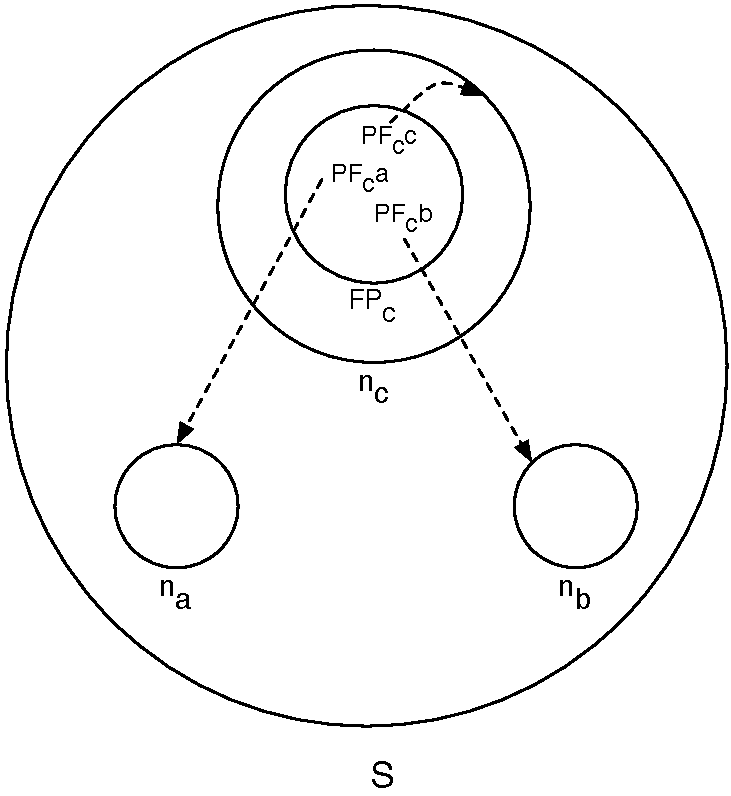
\includegraphics[width=0.60\textwidth]{images/precedence_filters.pdf}
  \caption{Diagram of relevant entities and data structures}
  \label{fig:precedence_filters}
\end{figure}

Our work is based in the decentralized approach. Both our
implementation and the tests we ran are based upon it. So,
from now on, we will be referring to the decentralized version only,
although it is not hard to draw conclusions that apply to the
centralized scenario as well.
With that in mind, Precedence Filters work as follows: supposing we
have a set of Bluetooth scanners (nodes) $S$, each node $n \in S$ has
a Precedence Filter $PF_n$. That PF is in turn composed of a set of
\emph{Counting Bloom Filters}, one for each node $z \in S$. We use
notation $PF_n^z$ to refer to the CBF for scanner $z$ belonging to
$PF_n$, as depicted in Figure ~\ref{fig:precedence_filters}.

All CBFs are initially set to 0, use the same set of hash functions
$K$ and have the same size $M = m * k$ ($k$ is calculated with
equation \ref{eq:optimal_hash_number} and $m$ is calculated with
equation \ref{eq:optimal_slice_size}). This ensures that the same
device is correctly identified across the several nodes (upon
detection it will be mapped to the same indices). Precedence Filters
can also be seen as a matrix where the number of rows is equal to the
number of nodes in the system and the number of columns is equal to $M$.

Each time a node $n$ detects a device $d$, its Precedence Filter
$PF_n$ is updated according to the following set of rules:
\begin{enumerate}
\item Using the set of hash functions $K$, the node $n$ calculates the
  set of indices $I_d$. $I_d$ consists on the output from the $K$ hash
  functions regarding device $d$, $I_d=\bigcup_{f \in K} f(d)$.
\item Node $n$ sends the set of indices $I_d$ to the all other nodes
  in $S$.
\item Each one of the $q$ nodes belonging to $Z$ ($Z = S \backslash
  \{n\}$) replies with a set of tuples $R_q$. $R_q$ contains
  the previously required $I_d$ along with the set of values that each
  of the CBFs belonging to $FP_z$ had stored in those indices,
  $R_q^{I_d}= (i,\{PF_z^x[i]\}) ,\forall i \in I_d, \forall x \in Z$
\item Upon the reception of the replied from the other nodes, $n$
  updates its own indices $I_d$ on the CBFs relative to the other
  nodes with the maximum value received, $PF_n^z[i] = \max(R_q[i][z] \forall
  q \in Z), \forall i \in I_d, \forall z \in Z$
\item Lastly, $n$ updates the indices $I_d$ on its own CBF
  ($PF_n^n$). For each index $i \in I_d, PF_n^n[i] = \max(PF_n^d[i])+1,
  \forall d \in S$. By adding 1 to the maximum value stored in the
  other nodes, the current node ``dominates'' them in the operation
  that returns the causality between the visited places. In other
  words, it is the key to obtaining the order in which the places were
  visited. 
\end{enumerate}

This set of rules allows the precedence filters to record information
about the precedence of the locals visited by a device. Given a set of
indices $I_d$ for device $d$ and any pair of scanners $x$ and $y$, we
say that the sighting of $d$ in $x$ precedes the one in $y$, $x
\leadsto y$ if: 

\begin{center}
\begin{math}
	x\leadsto y \Longleftrightarrow PF_{x}[I_d] < PF_{y}[I_d]
\end{math}
\end{center}
Where $PF_x[I_d] < PF_y[I_d]$ stands for:
\begin{center}
  \begin{math}
    \forall i \in I_d : PF_x^x[i] < PF_y^y[i]
  \end{math}

\end{center}
It is easy to see the similarities with the vector clock description
from Subsection \ref{sec:vector_clocks}. 

Mobility traces, used in our model to describe the behavior of
individuals, characterize a total order between the places
visited. This means that it is always possible to establish an order
between any two elements from the mobility trace. Being based upon the
happens-before relation~\cite{Lamport:1978}, Precedence Filters can
only represent partial orders. In this particular case, for each of
the nodes/locations they can only ``remember'' the last time each
device was sighted. For instance, given the mobility trace
$MT_{P}=\{S_1,S_2,S_1,S_3,S_2,S_4,S_1\}$ where places $S_1$ and $S_2$
are visited more than once, in the best case scenario PFs can obtain
$CT_{P}=\{S_3,S_2,S_4,S_1\}$, which we will refer as \emph{causality
 trace}. This is a consequence of the irreflexivity and antisymmetry
properties from the happens-before relation. However, we can look at
this as a feature of Precedence Filters, a sort of automatic data
degradation. It ensures that the record of sightings for any given
device has an upper bound equal to the number of Bluetooth scanners in
the tracking system.

The level of privacy offered by Precedence Filters can be further
customized by adjusting the CBFs' false positive ratio (Equation
\ref{eq:false_positive}). The higher the ratio, the greater the
inaccuracy of the PFs. The occurrence of false positives in the CBFs
results in the appearance of \emph{fictitious transitions}, i.e. the
causal trace obtained from querying the filters, contains transitions
which are non-existent in the original trace. 

Both these properties are what allow individual users to deny the
legitimacy of the data extracted from the Precedence Filters.


\section{Metrics and Data Sets}
\label{sec:metrics-data-sets}

To assess the performance of Precedence Filters we compare the set of
transitions obtained from querying the Precedence Filters with the set
of transitions obtained from the causality traces, which are themselves
obtained from mobility traces.  For instance, given the mobility trace
$MT_P=\{S_1,S_2,S_2,S_1,S_3\}$, we calculate its causality trace
$CT_P=\{S_2,S_1,S_3\}$, according to the happens-before relation (only
contains last sighting in each place). Then we extract a set of
transitions from that causality trace,
$\{(S_2,S_1),(S_2,S_3),(S_1,S_3)\}$. Each transition is a two location
tuple where the fist location causally precedes the second. In our
scenario, that means the device was seen in the first location
before being sighted at the second location. This
set of transitions is then finally compared a similar set of
transitions obtained from the PFs.


\subsubsection{Metrics}

The Precedence Filters performance is measured according to two
different metrics. The \emph{individual} metric which measures the
false probability of affirmations like the following - ``the
individual $P$ visited location $S_1$ before visiting location
$L2$''. This is done by calculating the cardinality of the mutually
exclusive set between the transitions belonging to the causality trace
($T_{CT}$) and the transitions extracted from the Precedence Filter
($T_{PF}$), according to Equation \ref{eq:individual_metric}.
 \begin{equation}
   \label{eq:individual_metric}
   \frac{ | (T_{CT} \bigcup T_{PF}) \backslash (T_{CT} \bigcap T_{PF}) | }{|T_{PF}|}
 \end{equation}

The \emph{global} metric quantifies the relative weight of one transition
(e.g. $(S_1,S_3)$) against the total number of transitions
recorded. For each type of transition, its total number of occurrences
is divided by the sum of total number of occurrences of all
transitions. By doing so we are able to establish the relative
importance of each type of transition, i.e. to make affirmations like
- ``2\% of the transitions are from Restaurant Y to Cafe X''. 

\subsubsection{Real Data set}

To evaluate the PFs' performance we used a real data set with
information about Bluetooth sightings by static nodes. This data set
was taken from Leguay et al. work~\cite{leguay2006opportunistic}. To
collect this information, the authors handed out a set of Bluetooth
enabled devices called \emph{iMotes} to a group of users who carried
them in their day-to-day. Additionally, the authors installed
Bluetooth scanners in several places with the purpose to register the
sighting of \emph{iMotes}. The dataset contains 18 static nodes and
9244 distinct device IDs, 6439 of which have been sighted only once
and were therefore removed. The average size for the mobility traces
is approximately 3 and the maximum size is 11. Figure
\ref{fig:dev_sig_real} shows the distribution of total and distinct
sightings for all scanners. As expected, not all places have the same
popularity, some are more visited than others, thus the bigger number
of Bluetooth sightings.

\begin{figure}[htb]
\subfigure[Real data set]{
  \label{fig:dev_sig_real} 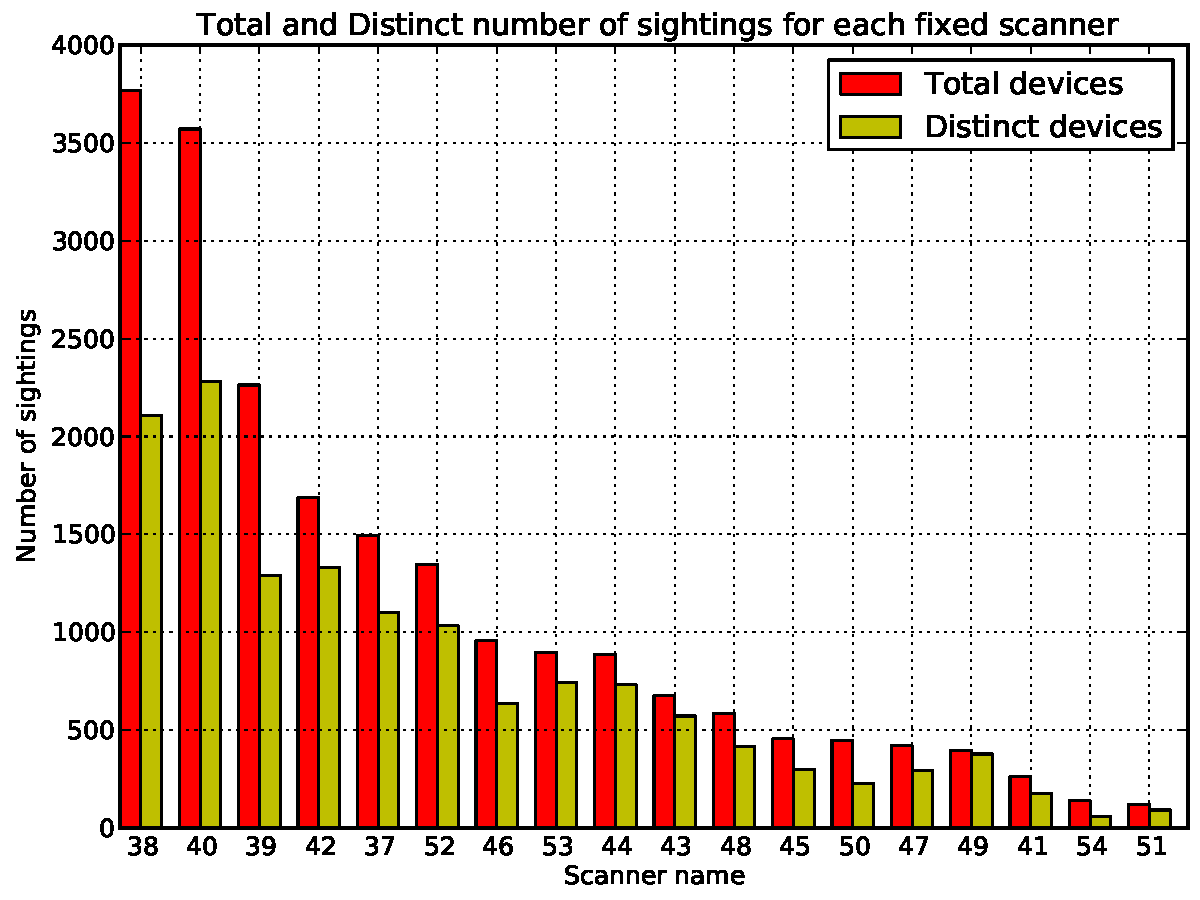
\includegraphics[scale=0.33]{images/rTotalDistinctSightings.pdf}
} \subfigure[Synthetic data set]{
 \label{fig:dev_sig_synthetic}  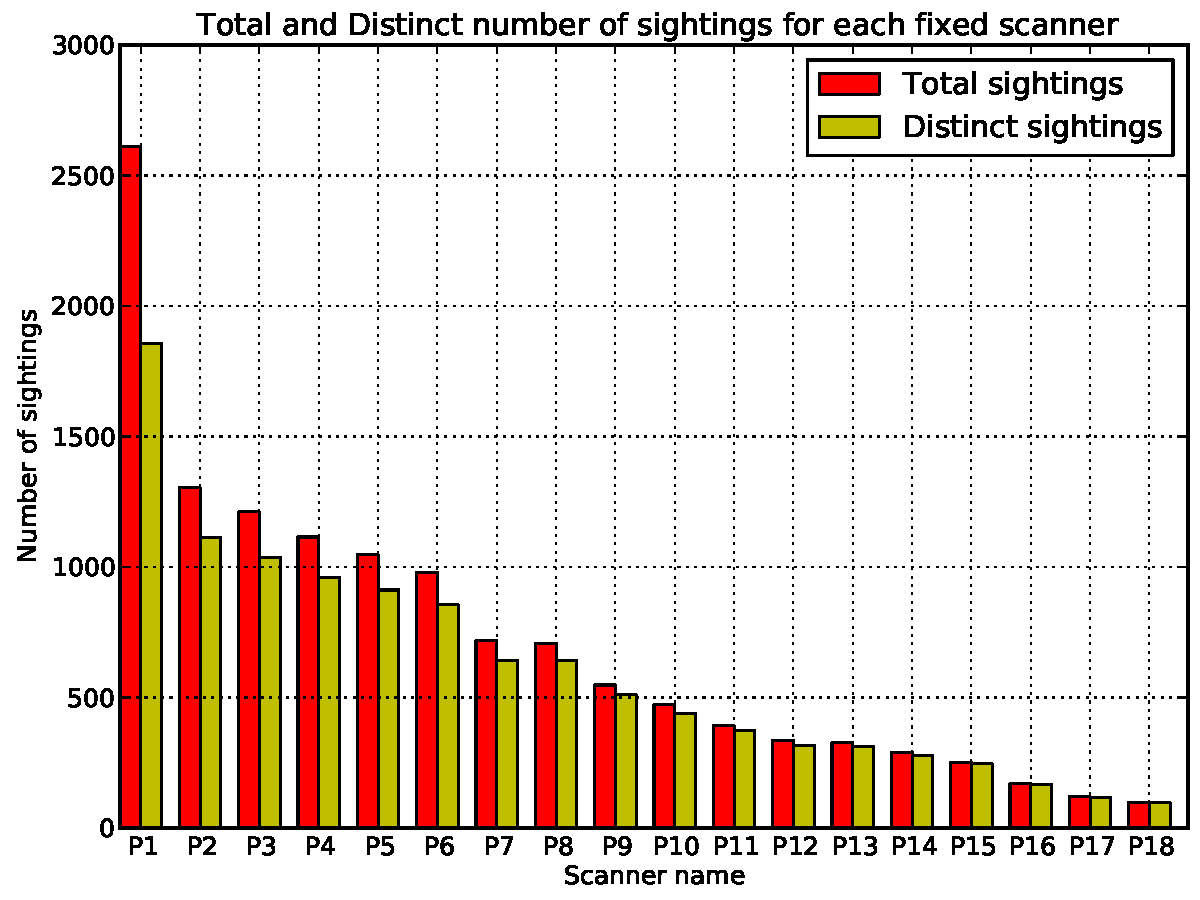
\includegraphics[scale=0.33]{images/sTotalDistinctSightings.pdf}
}
\caption{Number of total and distinct device sightings across the scanners}
\label{fig:deviceSightings}
\end{figure}

\subsubsection{Synthetic Data Set}
\label{sec:simulator}
Still in the context of evaluating the PF's performance, we built a
synthetic trace generator modeled after the real data set's
statistical distribution for the total number of sightings per place,
i.e. negative exponential distribution with $\lambda =
1132.44^{-1}$. Our motivation came from the need to simulate scenarios
with arbitrary number of locations and users. Our trace generator
allows us to choose the number of places, of users and the maximum
trace length to simulate. The real data set's mobility traces average
size is quite small. Figure \ref{fig:dev_sig_synthetic} shows the
synthetic distribution obtained with parameters similar to the ones
from the real data set. As expected the results are very similar but not a
perfect match, the curve from the synthetic data set is much smoother,
it does not suffer from the ``noise'' inherent to raw real data.


\section{Evaluation}
\label{sec:ct-evaluation}

Looking at Figure \todo{Resultado dataset} we can check that
precedence filters behave as expected. Increasing the false positive
probability of the Counting Bloom Filters leads to increasing
inaccuracy as well. This is true for both the individual and 
global metrics. 

\begin{figure}[htb]
\subfigure[Real data set]{
  \label{fig:dev_sig_real} 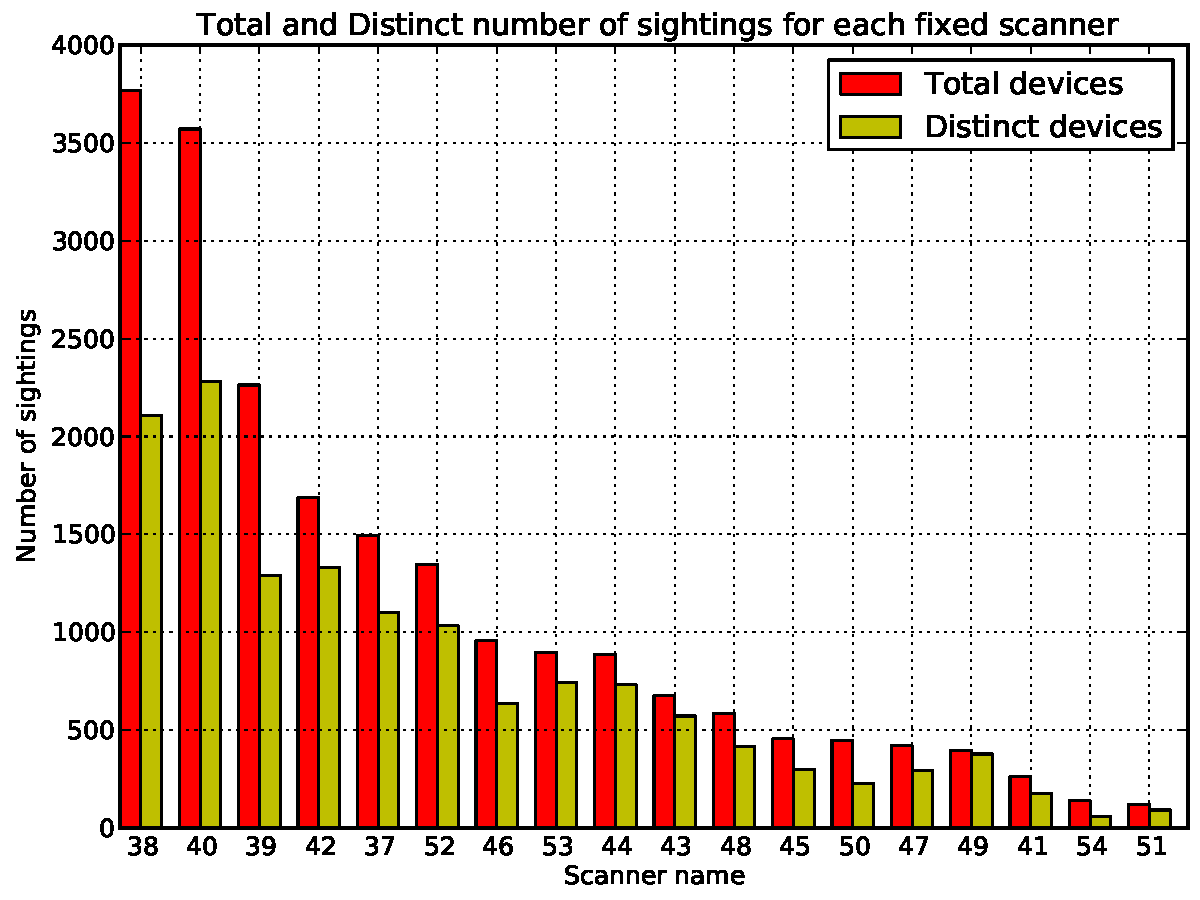
\includegraphics[scale=0.33]{images/rTotalDistinctSightings.pdf}
} \subfigure[Synthetic data set]{
 \label{fig:dev_sig_synthetic}  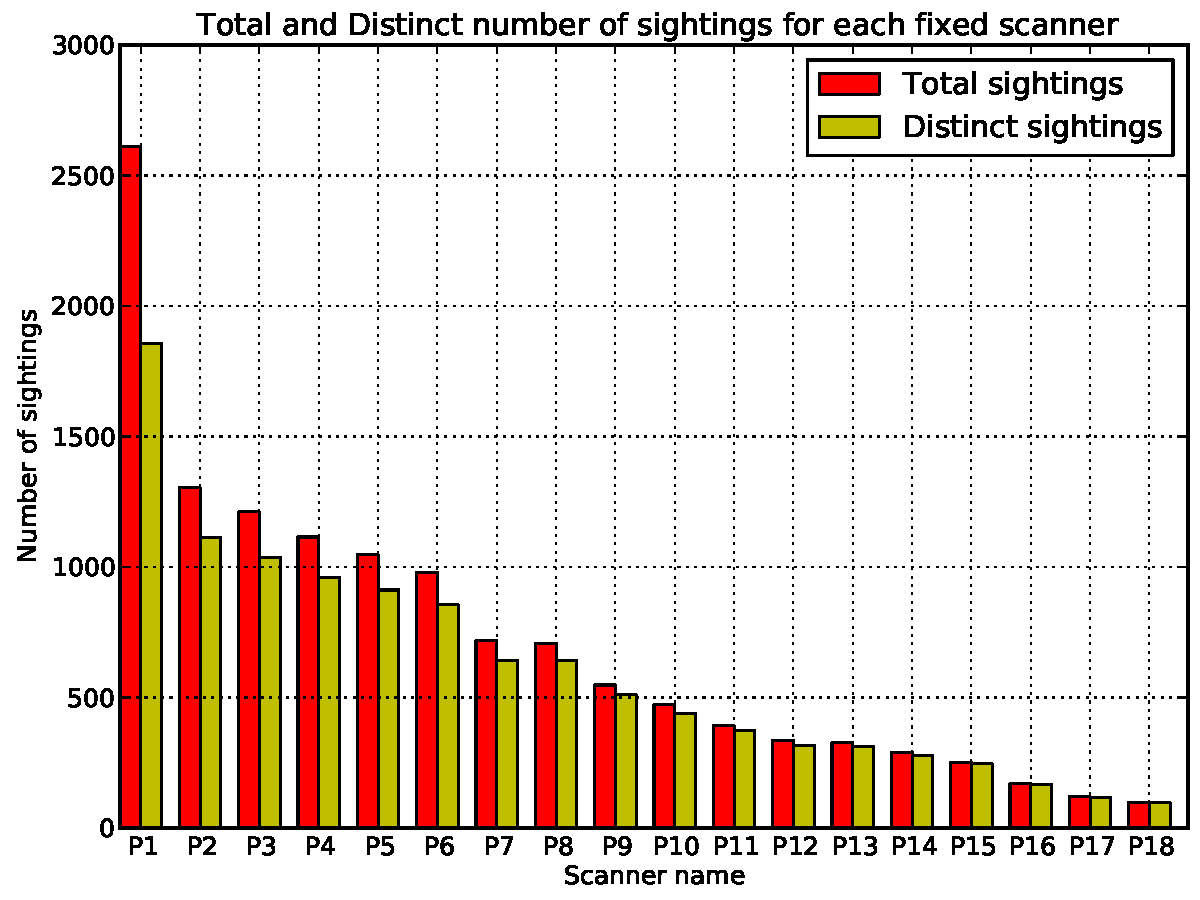
\includegraphics[scale=0.33]{images/sTotalDistinctSightings.pdf}
}
\caption{Number of total and distinct device sightings across the scanners}
\label{fig:deviceSightings}
\end{figure}

The inaccuracy is manifested via the occurrence of fake (PF only)
transitions, i.e. \emph{fictitious transitions}. As the false
probability increases, so does the percentage of fake
transitions. This easily explainable. In Bloom Filters, false
positives denote elements wrongfully considered as belonging to the
set. Given that in PFs, Bloom Filters are used to record device
sightings, false positives map to fake device sightings which in turn
give origin to fictitious transitions.

In Figure\todo{referencia dataset real}, for high false positive
probabilities ($\gtrsim$ 0.6), the global inaccuracy (dashed line) of our
mechanism is below the individual inaccuracy (solid line). This 

\section{Synopsis}
\label{sec:ct-synopsis}

%%% Local Variables: 
%%% mode: latex
%%% TeX-master: "../thesis"
%%% End: 
